% ══════════════════════════════════════════════════════════════════════════════
% How LLMs Process Information — A Geometric View
% 1-hour lecture deck
% ══════════════════════════════════════════════════════════════════════════════
\documentclass[aspectratio=169, 11pt]{beamer}

% ── Theme ────────────────────────────────────────────────────────────────────
\usetheme{metropolis}
\usepackage{appendixnumberbeamer}

% ── Packages ─────────────────────────────────────────────────────────────────
\usepackage{amsmath, amssymb}
\usepackage{graphicx}
\usepackage{booktabs}
\usepackage{tikz}
\usetikzlibrary{arrows.meta, positioning, decorations.pathmorphing, calc}
\usepackage{xcolor}
\usepackage{hyperref}

% ── Colors ───────────────────────────────────────────────────────────────────
\definecolor{Navy}{HTML}{1B2A4A}
\definecolor{Teal}{HTML}{0D7377}
\definecolor{Amber}{HTML}{D4A017}
\definecolor{DRed}{HTML}{9B2335}
\definecolor{DGreen}{HTML}{2E7D32}
\definecolor{Purple}{HTML}{6A1B9A}
\definecolor{LBlue}{HTML}{E3F2FD}

\setbeamercolor{frametitle}{bg=Navy, fg=white}
\setbeamercolor{progress bar}{fg=Teal}
\setbeamercolor{alerted text}{fg=DRed}

% ── Macros ───────────────────────────────────────────────────────────────────
\newcommand{\bivec}[1]{B^{(#1)}}
\newcommand{\rotor}[1]{R^{(#1)}}
\newcommand{\metric}[1]{P^{(#1)}}
\newcommand{\op}{\wedge}
\newcommand{\ip}{\cdot}

% ── Title ────────────────────────────────────────────────────────────────────
\title{How LLMs Process Information}
\subtitle{A Geometric View Inside Transformer Computation}
\author{Agus Sudjianto}
\date{\vspace{-1em}}
\institute{%
  \scriptsize Based on \emph{Learning Geometric Algebra Through Transformer Geometry}\\[1pt]
  \scriptsize\url{https://github.com/asudjianto-xml/layer-time-geometry}%
}

\begin{document}

% ══════════════════════════════════════════════════════════════════════════════
\begin{frame}[plain, noframenumbering]
\vspace{1.5cm}
{\Large\bfseries How LLMs Process Information}\\[4pt]
{\normalsize A Geometric View Inside Transformer Computation}

\vspace{0.8cm}
\textcolor{Teal}{\rule{0.4\textwidth}{0.8pt}}

\vspace{0.6cm}
{\normalsize Agus Sudjianto}

\vspace{0.4cm}
{\scriptsize Based on \emph{Learning Geometric Algebra Through Transformer Geometry}}\\[2pt]
{\scriptsize\url{https://github.com/asudjianto-xml/layer-time-geometry}}
\end{frame}

% ── Roadmap ──────────────────────────────────────────────────────────────────
\begin{frame}{Roadmap}
\begin{columns}[T]
\begin{column}{0.55\textwidth}
\begin{enumerate}
  \item \textbf{The Standard Picture} \hfill \textcolor{gray}{8 min}\\
    {\small Tokens, layers, hidden states}
  \item \textbf{Layers as Rotations} \hfill \textcolor{gray}{12 min}\\
    {\small Versors, bivectors, the metric as gauge}
  \item \textbf{When Order Matters} \hfill \textcolor{gray}{8 min}\\
    {\small Commutators, curvature, capacity}
  \item \textbf{The Decode Frontier} \hfill \textcolor{gray}{14 min}\\
    {\small Generation, directed flow, BCA}
  \item \textbf{Seeing Inside \& Steering} \hfill \textcolor{gray}{12 min}\\
    {\small Hallucination, monitoring, intervention}
  \item \textbf{Q\&A} \hfill \textcolor{gray}{6 min}
\end{enumerate}
\end{column}
\begin{column}{0.42\textwidth}
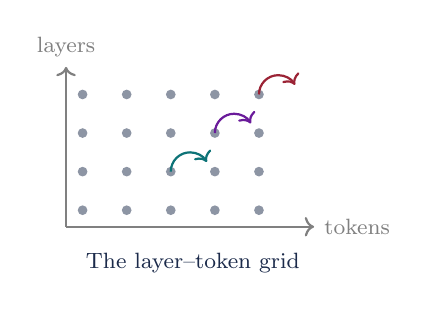
\begin{tikzpicture}[scale=0.7, every node/.style={font=\footnotesize}]
  % Grid dots
  \foreach \x in {0,...,4} {
    \foreach \y in {0,...,3} {
      \fill[Navy!50] (\x*0.8, \y*0.7) circle (2.5pt);
    }
  }
  % Axes
  \draw[->, gray, thick] (-0.3,-0.3) -- (4.2,-0.3) node[right] {tokens};
  \draw[->, gray, thick] (-0.3,-0.3) -- (-0.3,2.6) node[above] {layers};
  % Rotor arc
  \draw[->, Teal, thick] (1.6,0.7) arc[start angle=180, end angle=30, radius=0.35];
  \draw[->, Purple, thick] (2.4,1.4) arc[start angle=180, end angle=30, radius=0.35];
  \draw[->, DRed, thick] (3.2,2.1) arc[start angle=180, end angle=30, radius=0.35];
  \node[below, Navy] at (2.0, -0.6) {The layer--token grid};
\end{tikzpicture}
\end{column}
\end{columns}
\end{frame}


% ╔════════════════════════════════════════════════════════════════════════════╗
% ║  PART 1: THE STANDARD PICTURE                                           ║
% ╚════════════════════════════════════════════════════════════════════════════╝

\section{The Standard Picture}

% ── Slide: What happens when you prompt an LLM ──────────────────────────────
\begin{frame}{What happens when you prompt an LLM?}
\vspace{-0.2em}
\begin{center}
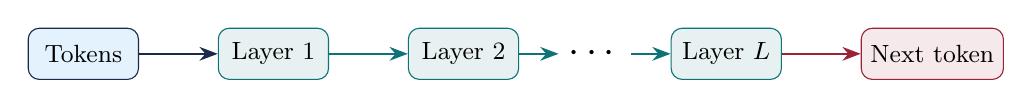
\begin{tikzpicture}[>=Stealth, node distance=1.0cm, font=\small]
  \node[draw=Navy, fill=LBlue, rounded corners, minimum width=1.4cm,
    minimum height=0.65cm] (tok) {Tokens};
  \node[draw=Teal, fill=Teal!10, rounded corners, minimum width=1.4cm,
    minimum height=0.65cm, right=of tok] (l1) {Layer 1};
  \node[draw=Teal, fill=Teal!10, rounded corners, minimum width=1.4cm,
    minimum height=0.65cm, right=of l1] (l2) {Layer 2};
  \node[right=0.5cm of l2, font=\Large] (dots) {$\cdots$};
  \node[draw=Teal, fill=Teal!10, rounded corners, minimum width=1.4cm,
    minimum height=0.65cm, right=0.5cm of dots] (lL) {Layer $L$};
  \node[draw=DRed, fill=DRed!10, rounded corners, minimum width=1.6cm,
    minimum height=0.65cm, right=of lL] (out) {Next token};
  \draw[->, thick, Navy] (tok) -- (l1);
  \draw[->, thick, Teal] (l1) -- (l2);
  \draw[->, thick, Teal] (l2) -- (dots);
  \draw[->, thick, Teal] (dots) -- (lL);
  \draw[->, thick, DRed] (lL) -- (out);
\end{tikzpicture}
\end{center}

\vspace{0.3em}
\begin{itemize}
  \item Each token becomes a \textbf{hidden-state vector} $H^{(l,t)} \in \mathbb{R}^{3584}$
  \item $L = 28$ layers, $T$ tokens $\Rightarrow$ a grid of $(28 \times T)$ vectors
  \item Standard view: ``matrix multiplies and attention.'' \alert{True but uninformative.}
\end{itemize}

\vspace{0.3em}
\begin{center}
\textbf{What is each layer actually \emph{doing} to these vectors?}
\end{center}
\end{frame}

% ── Slide: The layer-token grid ──────────────────────────────────────────────
\begin{frame}{The layer--token grid}
\begin{columns}[c]
\begin{column}{0.50\textwidth}
Every forward pass produces a \textbf{grid} of hidden states:
\[
  H : (l, t) \;\longmapsto\; \mathbb{R}^{p}
  \quad (p = 3584\text{ for Qwen2.5-7B})
\]
\vspace{-0.5em}
\begin{itemize}
  \item Vertical axis: \textbf{layers} ($L = 28$)
  \item Horizontal axis: \textbf{token positions} ($T$ tokens)
  \item Every dot is a high-dimensional vector
\end{itemize}

\vspace{0.3em}
{\small We need a language that describes not just \emph{how much} each layer changes the vectors, but \emph{in which directions}.}
\end{column}
\begin{column}{0.48\textwidth}
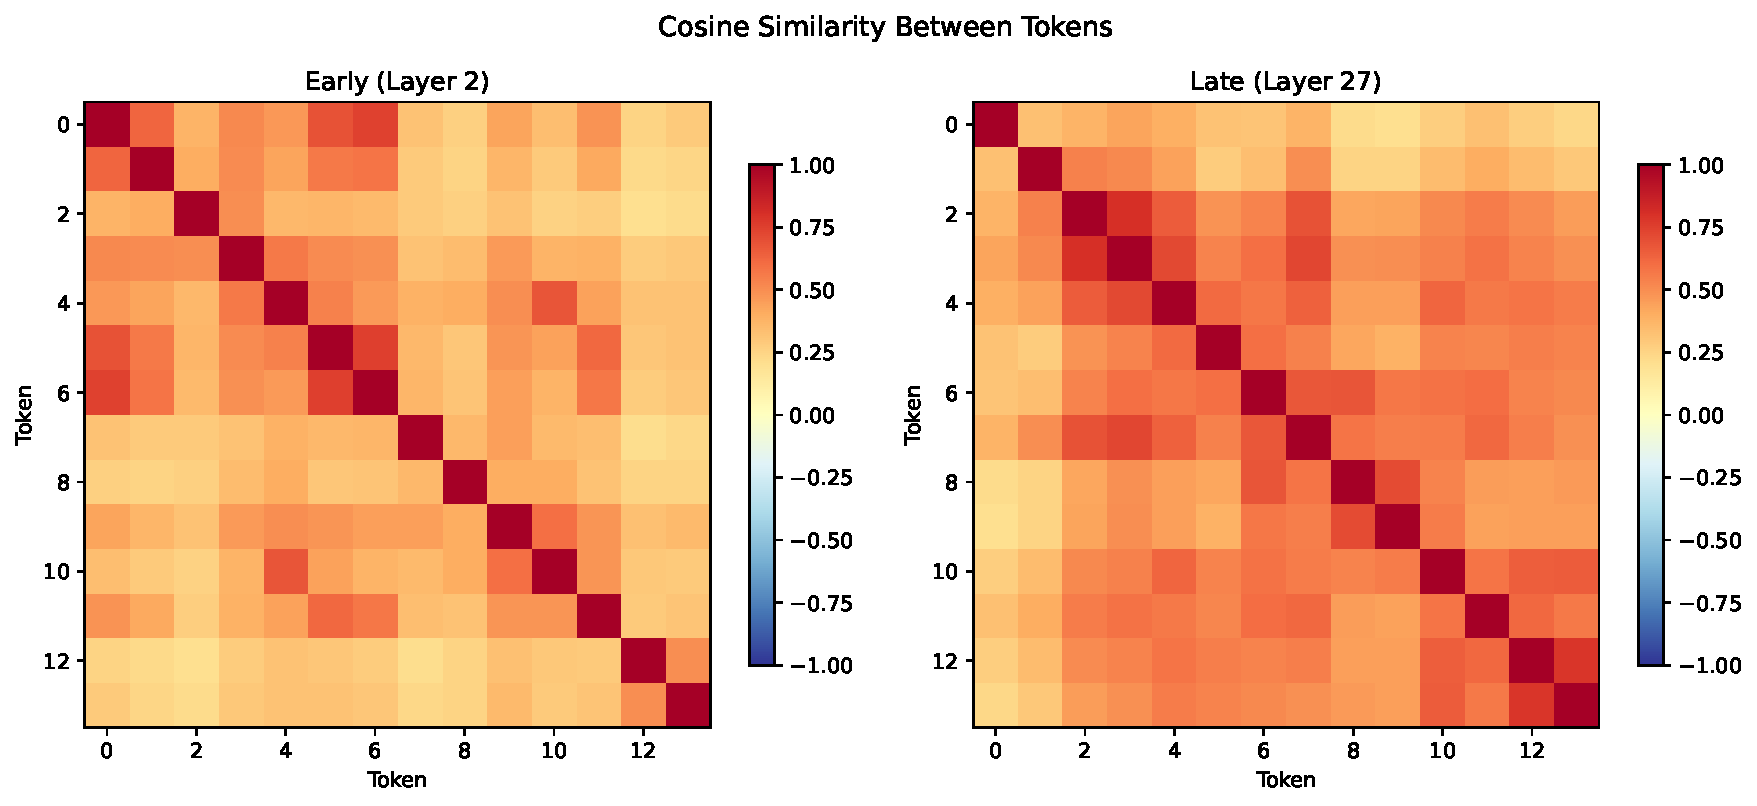
\includegraphics[width=\linewidth]{figures_ga_learning/ch01_cosine_layers.pdf}
\vspace{-0.3em}
{\scriptsize\textbf{Figure:} Cosine similarity between hidden states at adjacent layers. Values near 1 = small change; dips = layers that substantially redirect the vector. Each layer reshapes meaning by a different amount.}
\end{column}
\end{columns}
\end{frame}


% ╔════════════════════════════════════════════════════════════════════════════╗
% ║  PART 2: LAYERS AS ROTATIONS                                            ║
% ╚════════════════════════════════════════════════════════════════════════════╝

\section{Layers as Rotations}

% ── Slide: Whitening ─────────────────────────────────────────────────────────
\begin{frame}{Building an honest coordinate system}
\vspace{-0.3em}
{\small Raw hidden states live in $\mathbb{R}^{3584}$ with a \textbf{distorted} metric: distances and angles are unreliable.}

\vspace{-0.2em}
{\small\textbf{Whitening} (PCA + rescaling):}
\vspace{-0.5em}
\[
  \mathbb{R}^{3584} \;\xrightarrow{\text{PCA}}\; \mathbb{R}^{256}
  \;\xrightarrow{\text{rescale}}\; \text{Covariance} = I_{256}
\]

\vspace{-0.8em}
\begin{columns}[c]
\begin{column}{0.50\textwidth}
\begin{itemize}\small\setlength{\itemsep}{1pt}
  \item Retains $>99\%$ of variance
  \item Establishes an \textbf{orthonormal frame}
  \item Angles and rotations become \emph{meaningful}
  \item Acts as a \textbf{gauge}: the ``ruler'' for all
    subsequent measurements
\end{itemize}
\end{column}
\begin{column}{0.48\textwidth}
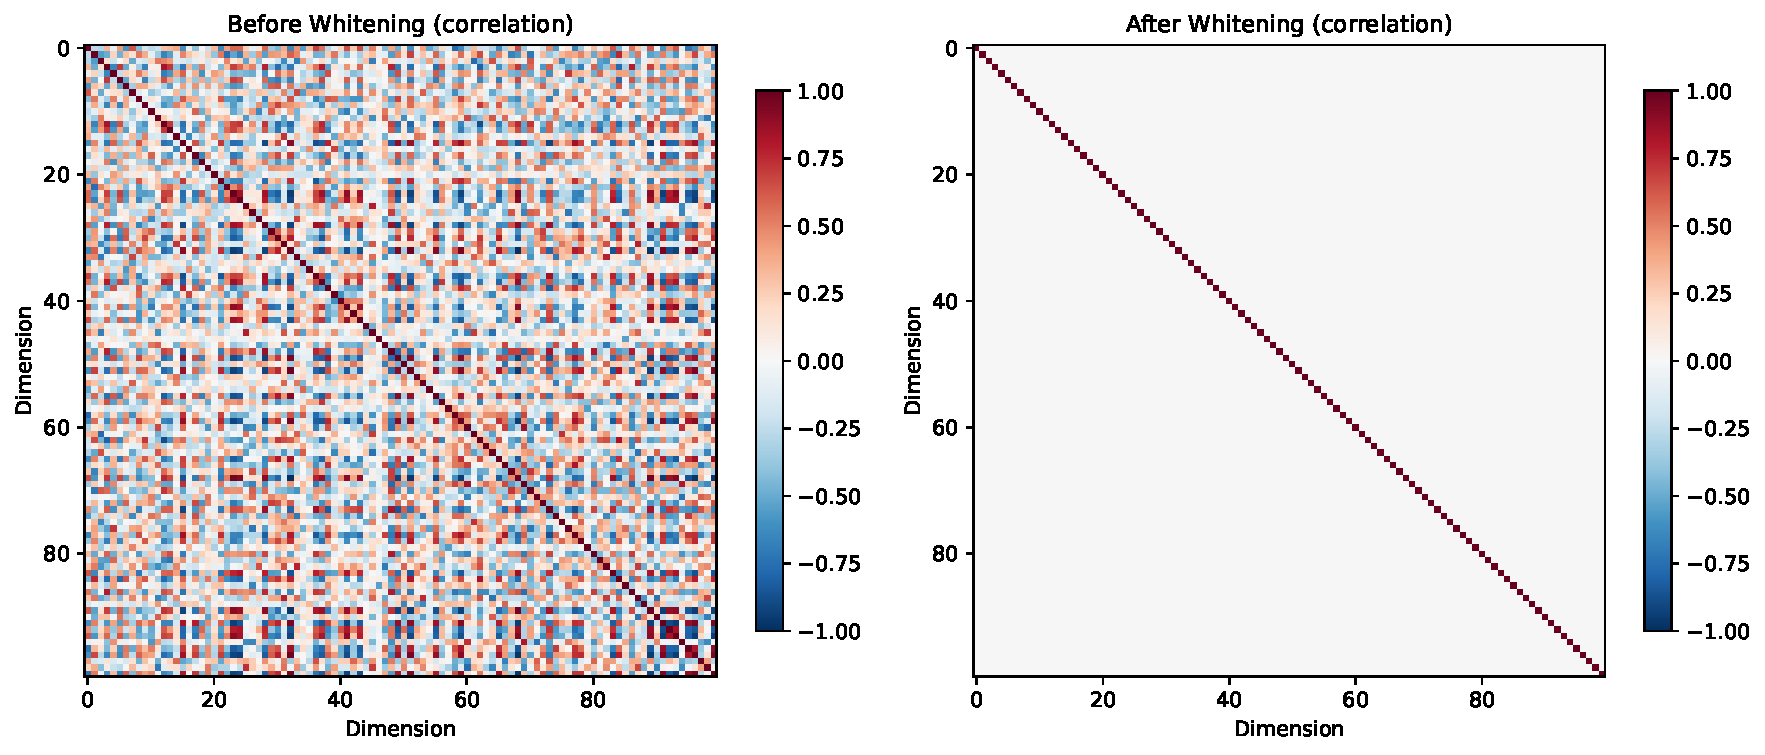
\includegraphics[width=\linewidth]{figures_ga_learning/ch04_covariance.pdf}
\vspace{-0.3em}
{\scriptsize\textbf{Figure:} Covariance structure before and after whitening. After whitening, the covariance is the identity --- distances and angles become trustworthy.}
\end{column}
\end{columns}
\end{frame}

% ── Slide: The versor decomposition ──────────────────────────────────────────
\begin{frame}{What a layer does: rotation $\times$ stretch}

Each layer transition (averaged across token positions) decomposes as:
\[
  \boxed{T^{(l)} \;=\; \underbrace{\rotor{l}}_{\text{rotation}} \;\cdot\; \underbrace{\metric{l}}_{\text{stretch}}}
\]
\vspace{-0.3em}
{\scriptsize (Attention makes $T$ position-dependent; we'll see per-token rotors on the next slides.)}

\begin{columns}[T]
\begin{column}{0.48\textwidth}
\textbf{Rotation} (grade-2, rotor)
\begin{itemize}
  \item Reorients the hidden state --- moves meaning to \emph{different directions}
  \item Preserves vector lengths
  \item Generator: bivector $\bivec{l} = \log(\rotor{l})$
\end{itemize}
\end{column}
\begin{column}{0.48\textwidth}
\textbf{Stretch} (grade-0, metric factor)
\begin{itemize}
  \item Amplifies or suppresses specific components --- \emph{adjusts emphasis}
  \item Preserves directions
  \item Near-identity in practice
\end{itemize}
\end{column}
\end{columns}

\vspace{0.3em}
\begin{center}
\alert{Empirical finding (Qwen2.5-7B):} Rotation dominates stretch by \textbf{10--15$\times$} in norm.\\
\textbf{Layers mostly rotate} --- they redirect meaning, not rescale it.
\end{center}

\vspace{-0.3em}
{\scriptsize\textcolor{gray}{Connection: $T^{(l)} \approx \partial H^{(l+1)}/\partial H^{(l)}$ --- the versor \emph{is} the layer Jacobian.  Rotation = reorientation of meaning; stretch = gain control.}}
\end{frame}

% ── Slide: Grade profile ─────────────────────────────────────────────────────
\begin{frame}{Rotation dominates: the grade profile}
\begin{center}
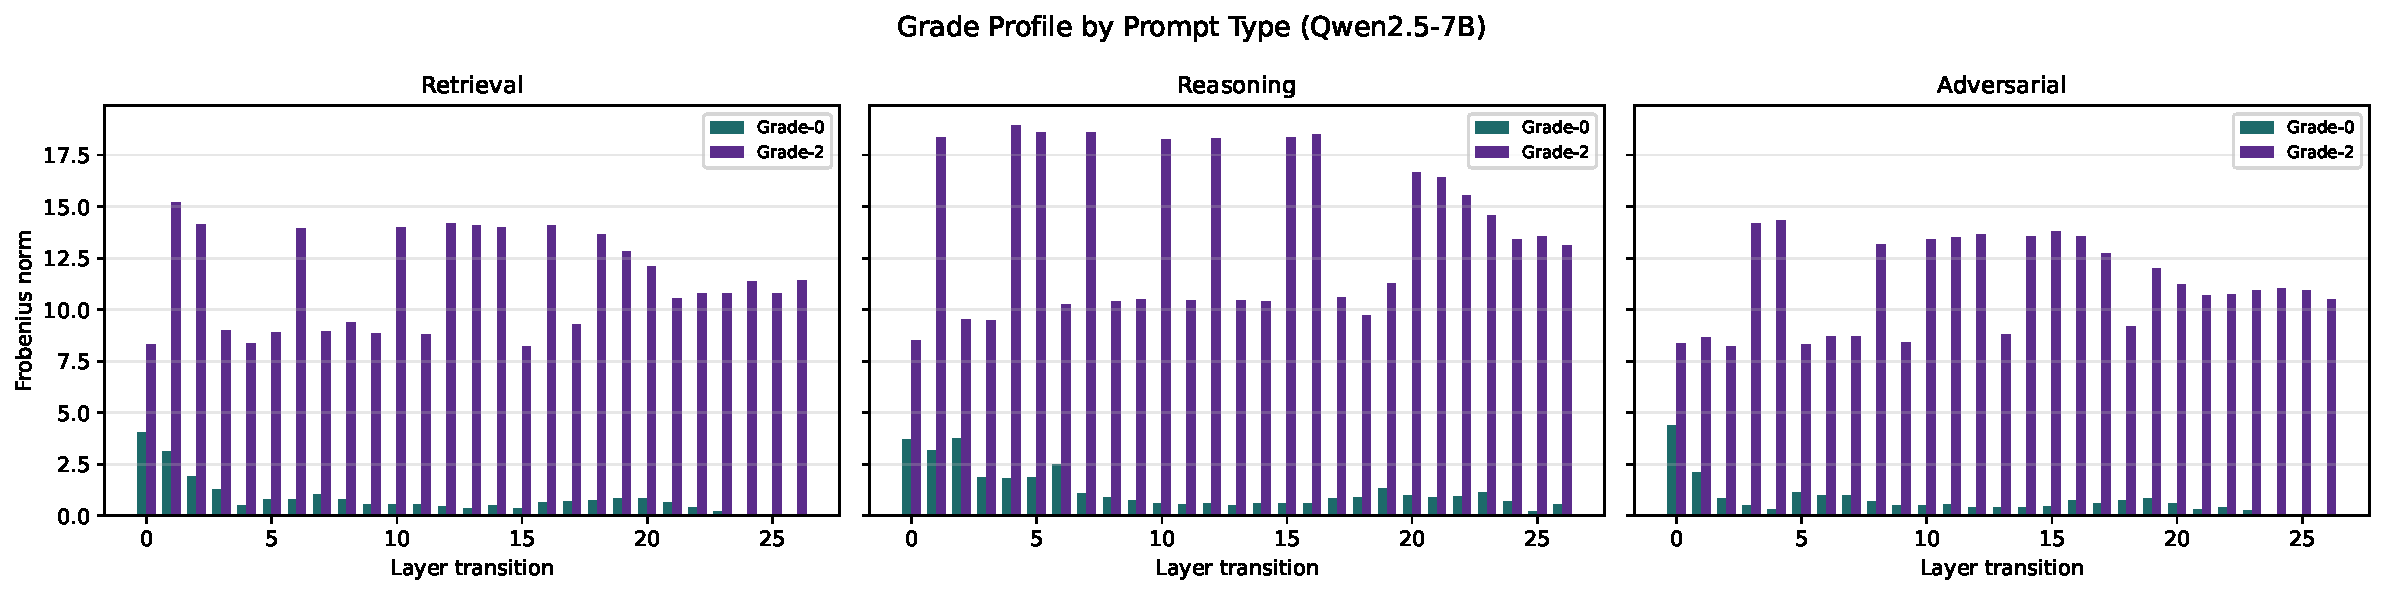
\includegraphics[width=0.78\linewidth]{figures_ga_learning/ch06_grade_profile_3prompts.pdf}
\end{center}

\vspace{-0.5em}
{\small
Blue = rotation (grade-2) norm; purple = stretch (grade-0) norm, per layer and prompt type.
Rotation outweighs stretch by \textbf{10--15$\times$} at every layer --- layers reshape \emph{which directions} matter, not how big they are.}
\end{frame}

% ── Slide: Bivectors — the plane of rotation ─────────────────────────────────
\begin{frame}{Bivectors: the plane of rotation}
\vspace{-0.3em}
{\small A rotation in $\mathbb{R}^{256}$ doesn't have an ``axis.'' It has a \textbf{plane}.}

\vspace{-0.1em}
\begin{columns}[c]
\begin{column}{0.55\textwidth}
{\small The bivector $\bivec{l} = \log(\rotor{l})$ is a \textbf{skew-symmetric matrix} encoding:}
\begin{itemize}\small\setlength{\itemsep}{1pt}
  \item \textbf{Which plane(s)} the layer rotates in
  \item \textbf{How much} (the angle $\theta$)
\end{itemize}

\vspace{0.2em}
{\small Principal plane decomposition:
$\bivec{l} = \sum_{j=1}^{128} \sigma_j \;\hat{B}_j$.
Typically \textbf{3--5 dominant planes} per layer.}
\end{column}
\begin{column}{0.43\textwidth}
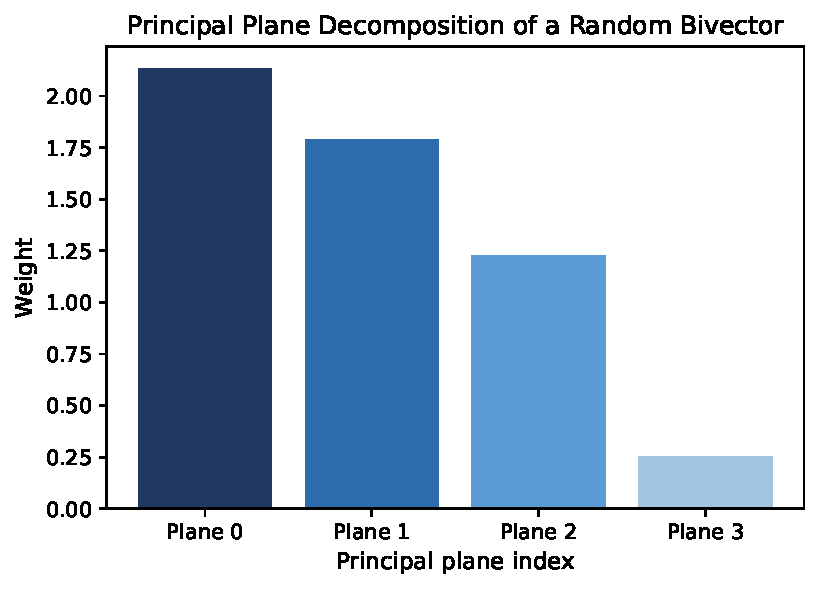
\includegraphics[width=\linewidth]{figures_ga_learning/ch03_principal_planes.pdf}
\vspace{-0.3em}
{\scriptsize\textbf{Figure:} Singular values of the bivector. The first few bars dominate --- rotation is concentrated in 3--5 planes, not all 128.}
\end{column}
\end{columns}
\end{frame}

% ── Slide: The rotor field ───────────────────────────────────────────────────
\begin{frame}{A layer is a \emph{field} of rotations}

Attention makes the transformation \textbf{position-dependent}:
\[
  H^{(l+1)}(t) \;=\; \rotor{l}(t)\;\metric{l}(t)\;\; H^{(l)}(t)
\]

Each token position gets its \textbf{own rotor}.

\begin{center}
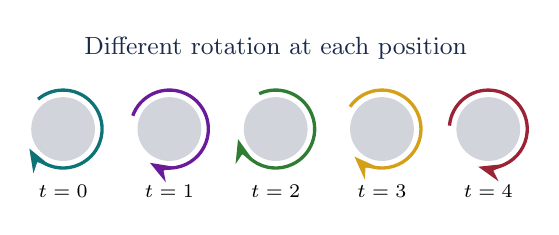
\begin{tikzpicture}[>=Stealth, scale=0.9]
  \foreach \i/\col/\ang in {0/Teal/40, 1/Purple/70, 2/DGreen/25, 3/Amber/55, 4/DRed/85} {
    \fill[Navy!20] (\i*1.5, 0) circle (0.45);
    \draw[->, \col, thick, line width=1.2pt]
      ([shift={(90+\ang:0.55)}]\i*1.5, 0)
      arc[start angle=90+\ang, end angle=90+\ang-280, radius=0.55];
    \node[below, font=\scriptsize] at (\i*1.5, -0.65) {$t = \i$};
  }
  \node[above, font=\small, Navy] at (3.0, 0.85) {Different rotation at each position};
\end{tikzpicture}
\end{center}

\vspace{0.3em}
A layer is not ``a rotation'' --- it is a \textbf{field of rotors},
each rotating the hidden state in its own plane by its own angle.
\end{frame}

% ── Slide: Rotor angles across layers ────────────────────────────────────────
\begin{frame}{Rotor angles across layers}
\vspace{-0.5em}
\begin{center}
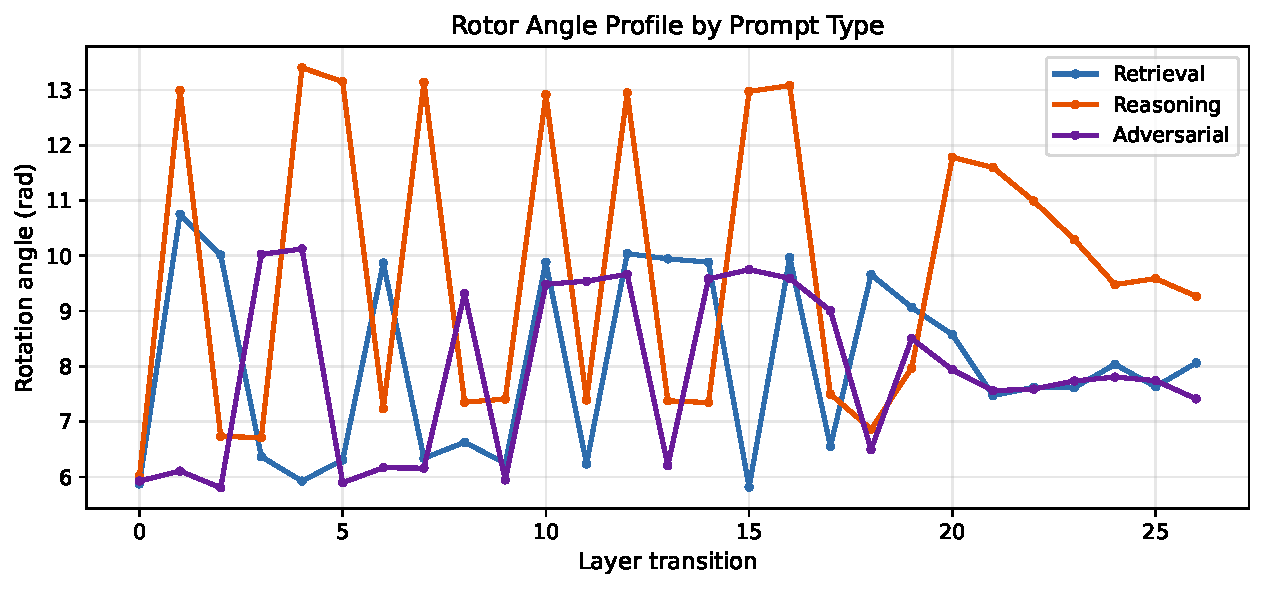
\includegraphics[width=0.70\linewidth]{figures_ga_learning/ch06_rotor_angles_3prompts.pdf}
\end{center}

\vspace{-0.8em}
{\footnotesize
\textbf{Reading the figure:} Each curve traces rotation angle $\tau^{(l)}$ (degrees) per layer for one prompt type. Higher = bigger rotation.
\textbf{Takeaway:} Early layers rotate aggressively ($40$--$60^{\circ}$); deeper layers make finer adjustments. Different tasks produce \emph{different} profiles --- the model adapts its rotation schedule to the input.}
\end{frame}


% ╔════════════════════════════════════════════════════════════════════════════╗
% ║  PART 3: WHEN ORDER MATTERS                                             ║
% ╚════════════════════════════════════════════════════════════════════════════╝

\section{When Order Matters}

% ── Slide: Commutators ───────────────────────────────────────────────────────
\begin{frame}{Do layers commute?}
\vspace{-0.5em}
{\small The \textbf{commutator} asks: does it matter which order I apply two layers' rotations?}
\vspace{-0.3em}
\[
  [\bivec{l},\; \bivec{l+1}] \;=\; \bivec{l}\bivec{l+1} - \bivec{l+1}\bivec{l}
\]
\vspace{-1em}
\begin{columns}[T]
\begin{column}{0.50\textwidth}
\begin{itemize}\small\setlength{\itemsep}{2pt}
  \item $= 0$: layers are \textbf{independent} ---
    swapping them wouldn't change the result
  \item $\neq 0$: layer $l{+}1$ \textbf{builds on} layer $l$'s
    rotation --- sequential processing matters
  \item Non-zero commutator = \emph{genuinely sequential} reasoning, not parallel operations
\end{itemize}
\end{column}
\begin{column}{0.48\textwidth}
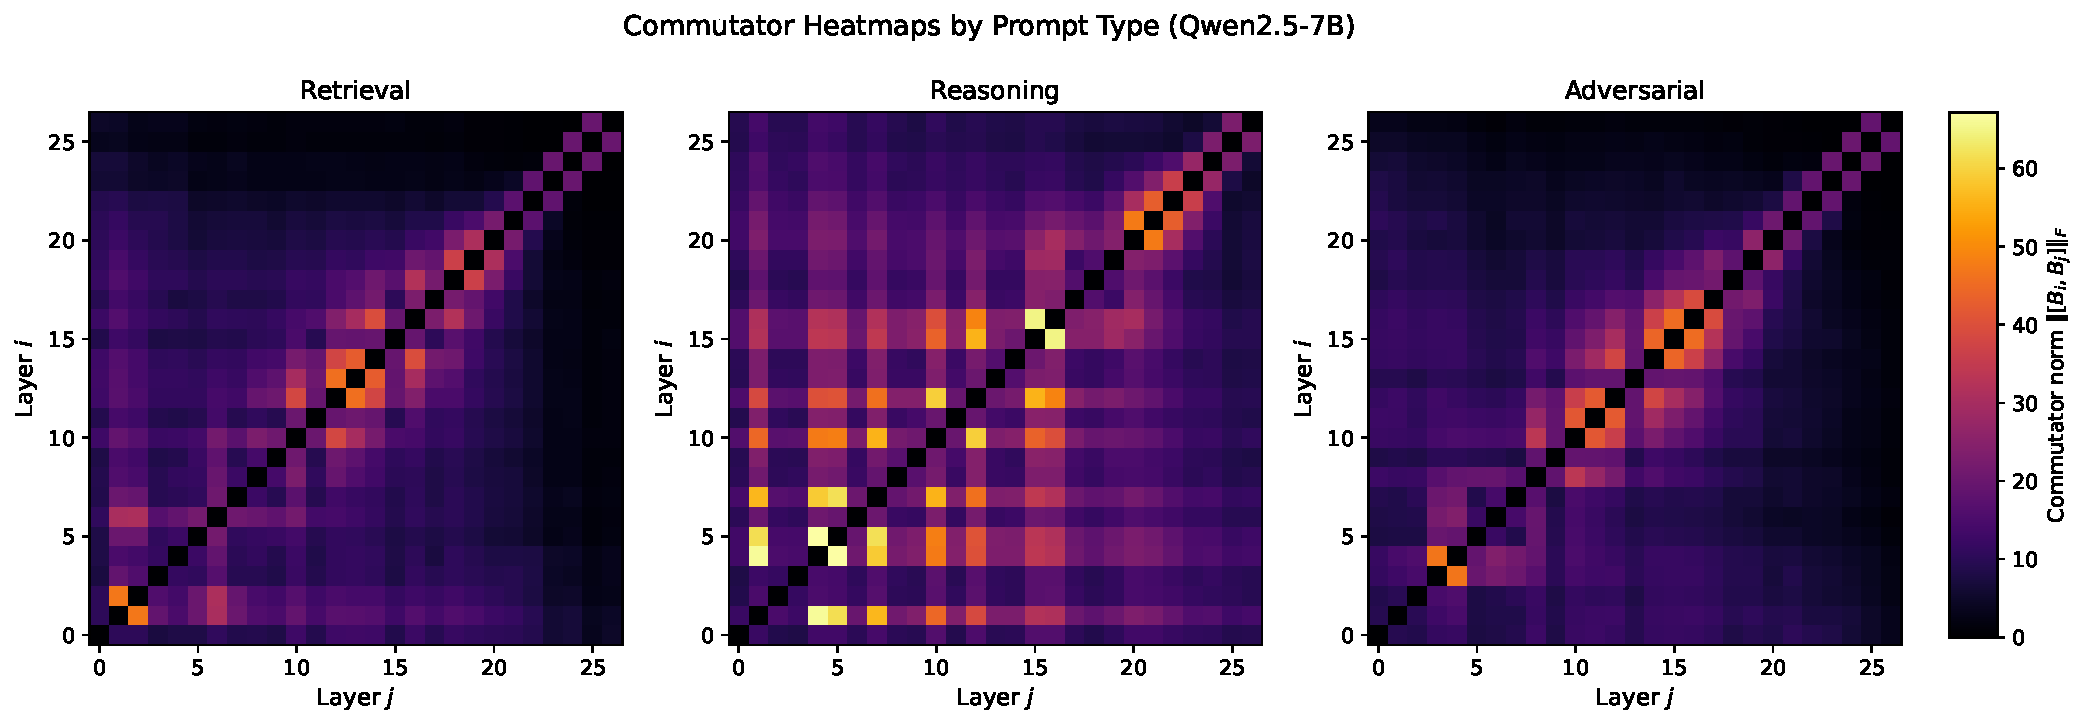
\includegraphics[width=\linewidth]{figures_ga_learning/ch09_commutator_3prompts.pdf}
\vspace{-0.3em}
{\scriptsize\textbf{Figure:} Commutator norm $\|[\bivec{l}, \bivec{l+1}]\|_F$ per layer pair. Higher = stronger sequential coupling.}
\end{column}
\end{columns}
\end{frame}

% ── Slide: Capacity ──────────────────────────────────────────────────────────
\begin{frame}{Capacity: the model's non-commutative budget}
\vspace{-0.5em}
{\small \textbf{Capacity} = total sequential computation. Sum commutator norms over all adjacent layer pairs:}
$C_{\text{acc}} = \sum_{\text{adj.\ pairs}} \|[\bivec{l}, \bivec{l+1}]\|_F$

\vspace{-0.2em}
\begin{columns}[c]
\begin{column}{0.48\textwidth}
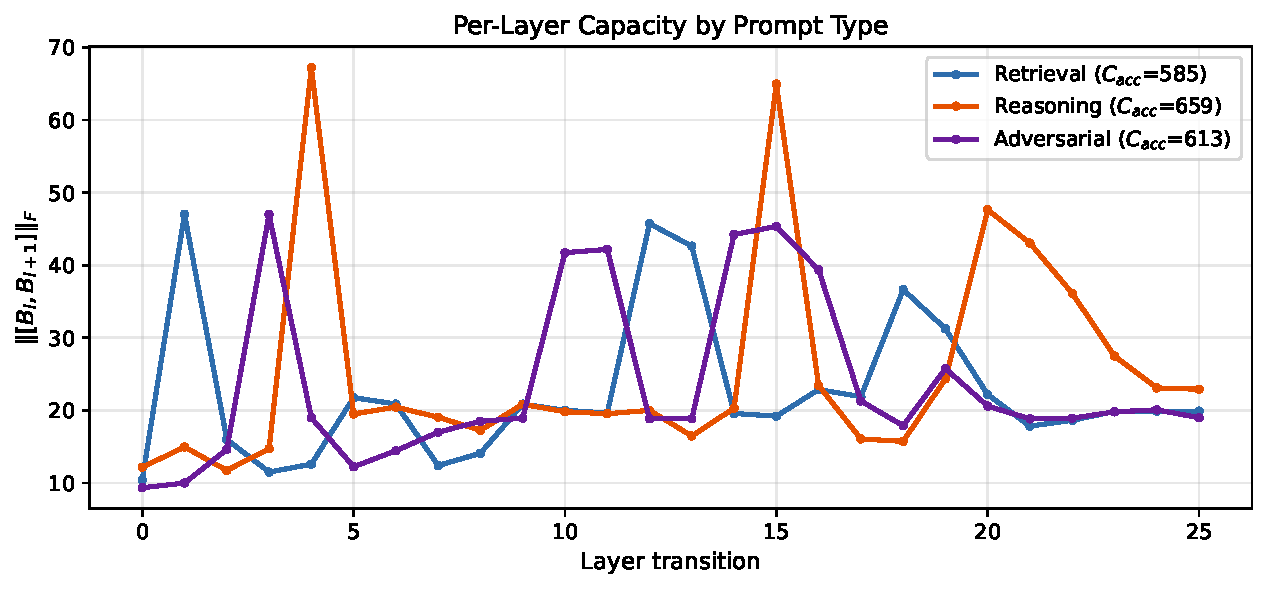
\includegraphics[width=\linewidth]{figures_ga_learning/ch11_capacity_3prompts.pdf}
\vspace{-0.3em}
{\scriptsize\textbf{Figure:} Cumulative capacity $C_{\text{acc}}$ vs.\ layer. Steeper climb = more sequential computation invested up to that depth.}
\end{column}
\begin{column}{0.48\textwidth}
\begin{center}
\renewcommand{\arraystretch}{1.1}\small
\begin{tabular}{@{} l r r @{}}
\toprule
\textbf{Prompt} & $C_{\text{acc}}$ & \textbf{Peak} \\
\midrule
Retrieval   & 584.9 & Layer 1 \\
Reasoning   & 658.5 & Layer 4 \\
Adversarial & 613.4 & Layer 3 \\
\bottomrule
\end{tabular}
\end{center}

\vspace{0.2em}
\begin{itemize}\small\setlength{\itemsep}{2pt}
  \item Reasoning demands \textbf{13\% more} capacity --- more sequential steps needed
  \item Peak layer shifts with task: the model allocates its ``budget'' \textbf{adaptively}
\end{itemize}
\end{column}
\end{columns}
\end{frame}

% ── Slide: Holonomy ──────────────────────────────────────────────────────────
\begin{frame}{Walking in circles: holonomy and curvature}
\vspace{-0.5em}
{\small Transport a vector around a closed loop on the grid. If it comes back \emph{changed}, the space is curved.}
\vspace{-0.3em}
\begin{columns}[c]
\begin{column}{0.46\textwidth}
\begin{center}
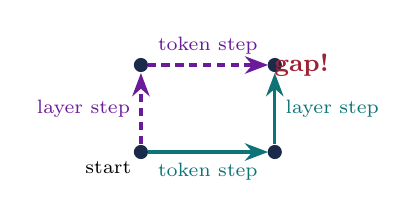
\begin{tikzpicture}[>=Stealth, scale=0.85]
  \foreach \x/\y in {0/0, 2/0, 0/1.3, 2/1.3} {
    \fill[Navy] (\x, \y) circle (3pt);
  }
  \draw[->, Teal, very thick] (0.1, 0) -- (1.9, 0)
    node[midway, below, font=\scriptsize] {token step};
  \draw[->, Teal, very thick] (2, 0.12) -- (2, 1.18)
    node[midway, right, font=\scriptsize] {layer step};
  \draw[->, Purple, very thick, densely dashed] (0, 0.12) -- (0, 1.18)
    node[midway, left, font=\scriptsize] {layer step};
  \draw[->, Purple, very thick, densely dashed] (0.1, 1.3) -- (1.9, 1.3)
    node[midway, above, font=\scriptsize] {token step};
  \node[DRed, font=\small\bfseries] at (2.4, 1.3) {gap!};
  \node[below left, font=\scriptsize] at (0, 0) {start};
\end{tikzpicture}
\end{center}
\end{column}
\begin{column}{0.50\textwidth}
{\small Compose all four rotors around the cell --- the \textbf{loop rotor}:}
\vspace{-0.3em}
\[
  R_{\text{loop}} = R_\uparrow \, R_\rightarrow \, R_\uparrow^{-1} R_\rightarrow^{-1}
\]
\vspace{-0.8em}

{\small If $R_{\text{loop}} \neq I$: the grid is \textbf{curved}.
$\Omega = \log(R_{\text{loop}})$ tells you \emph{which plane}.}

\vspace{0.2em}
{\small\alert{Intuition:} how a layer transforms a token \emph{depends on which other tokens it has seen} --- layer and context are entangled.}
\end{column}
\end{columns}
\end{frame}

% ── Slide: Holonomy empirical ────────────────────────────────────────────────
\begin{frame}{Curvature across the grid}
\vspace{-0.3em}
\begin{center}
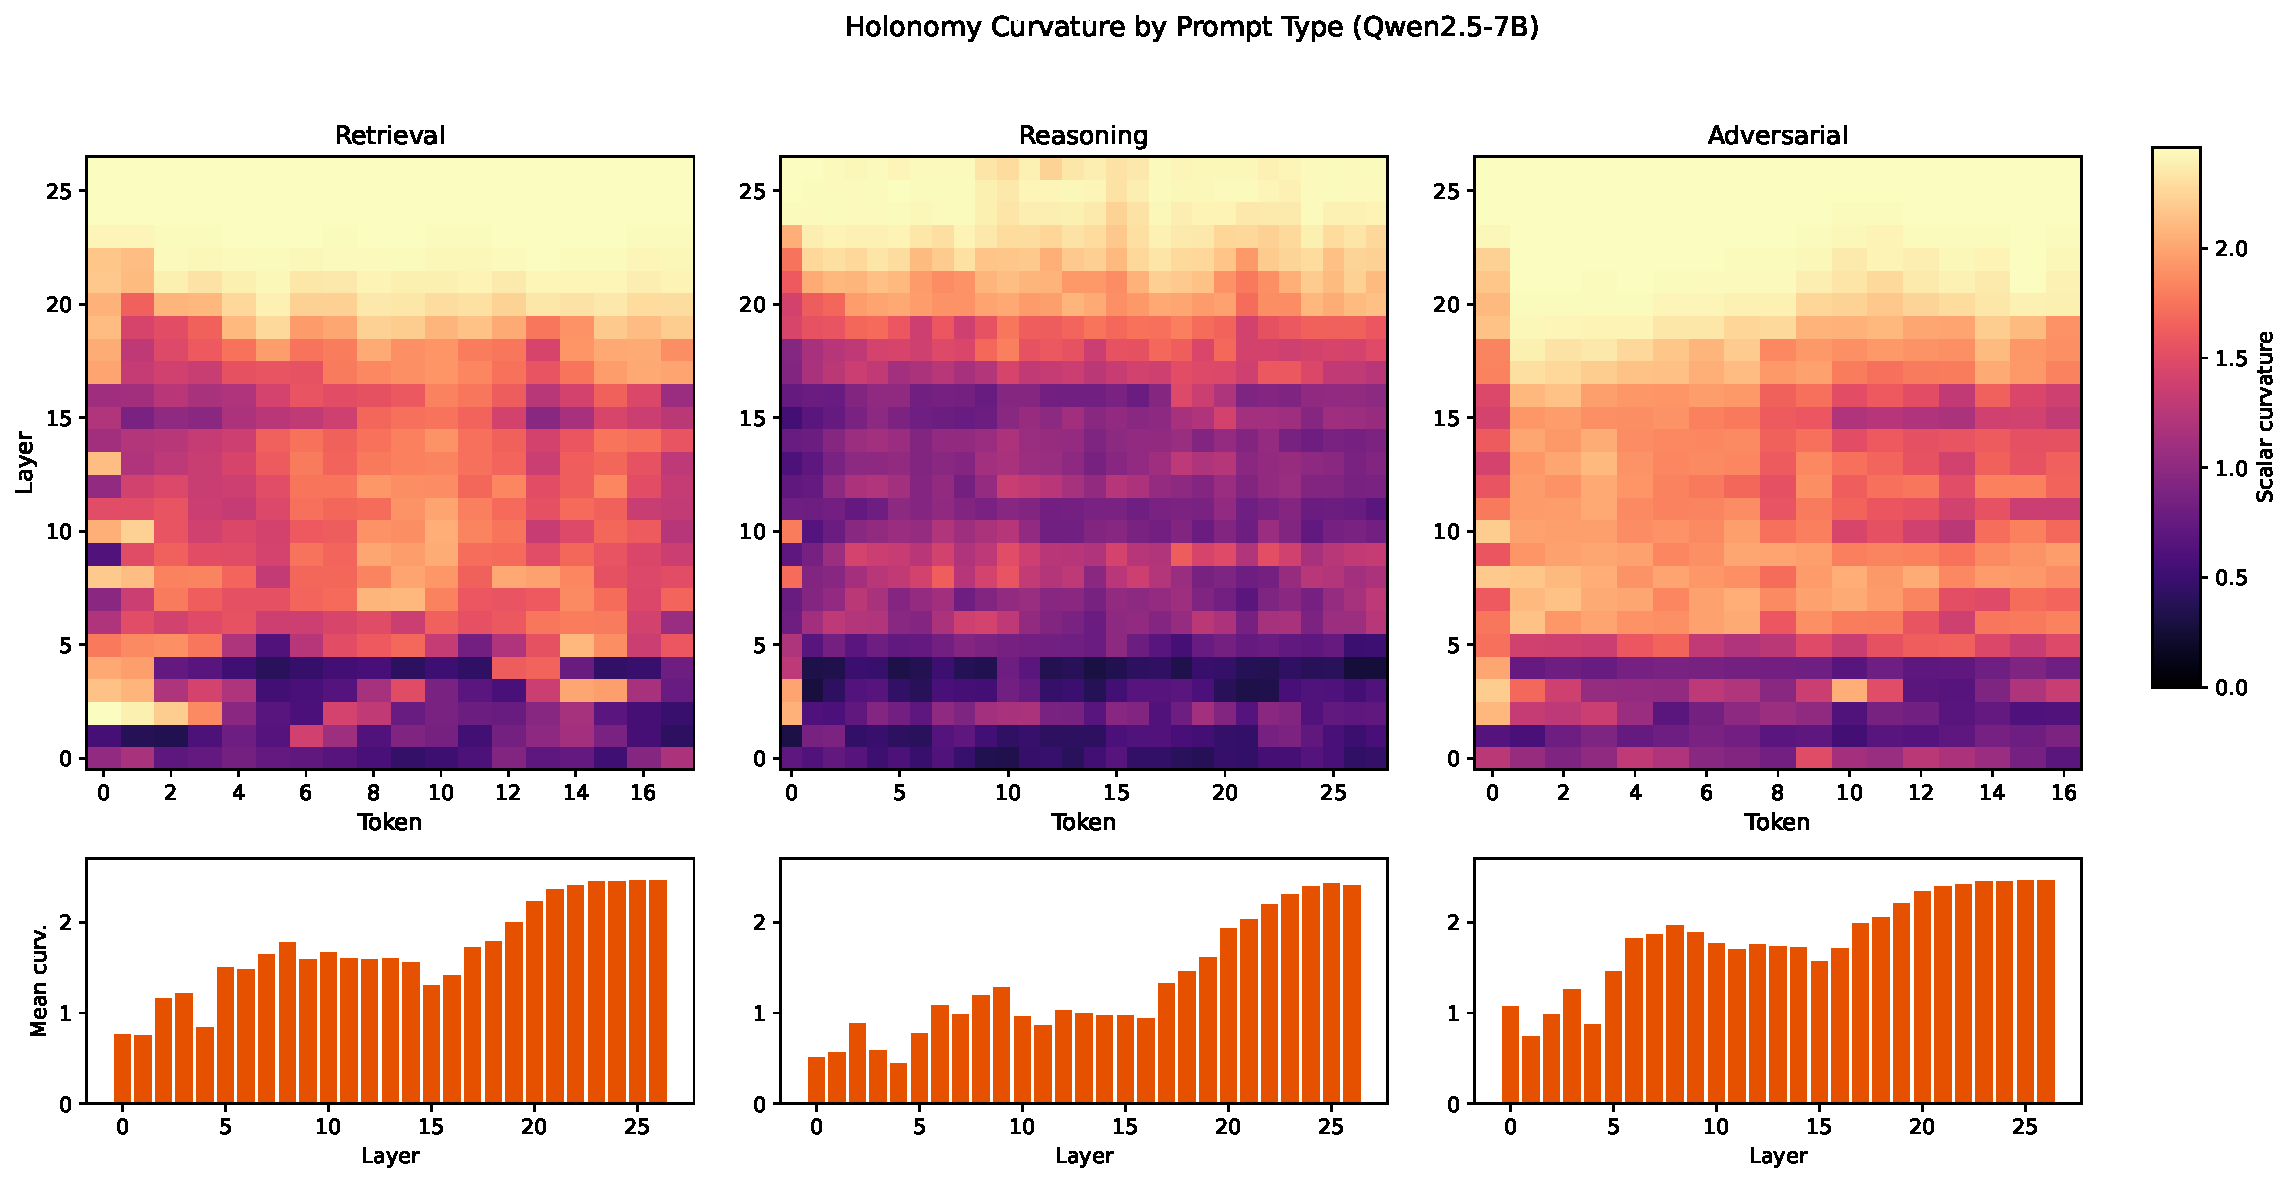
\includegraphics[width=0.70\linewidth]{figures_ga_learning/ch10_holonomy_3prompts.pdf}
\end{center}

\vspace{-0.8em}
{\footnotesize
\textbf{Reading the figure:} Each heatmap cell is one plaquette $(l, t)$. Color intensity = holonomy deficit $\|R_{\text{loop}} - I\|_F$. Brighter = more curvature.
\textbf{Takeaway:} Non-zero curvature means layer and token processing are \textbf{entangled}. Reasoning prompts show the strongest curvature.}
\end{frame}


% ╔════════════════════════════════════════════════════════════════════════════╗
% ║  PART 4: THE DECODE FRONTIER                                            ║
% ╚════════════════════════════════════════════════════════════════════════════╝

\section{The Decode Frontier}

% ── Slide: Static vs. dynamic ────────────────────────────────────────────────
\begin{frame}{From static analysis to generation}
\vspace{-0.2em}
Everything so far: one prompt, one forward pass.
But LLMs \textbf{generate} --- one token at a time.

\begin{center}
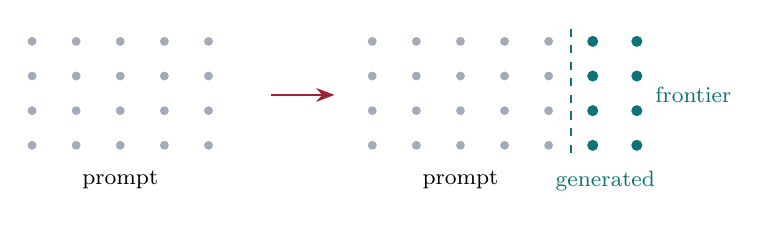
\begin{tikzpicture}[>=Stealth, scale=0.8, font=\small]
  \foreach \x in {0,...,4} {
    \foreach \y in {0,...,3} {
      \fill[Navy!40] (\x*0.7, \y*0.55) circle (2pt);
    }
  }
  \node[below, font=\footnotesize] at (1.4, -0.25) {prompt};
  \draw[->, thick, DRed] (3.8, 0.8) -- (4.8, 0.8);
  \foreach \x in {0,...,4} {
    \foreach \y in {0,...,3} {
      \fill[Navy!40] (5.4+\x*0.7, \y*0.55) circle (2pt);
    }
  }
  \foreach \x in {5,6} {
    \foreach \y in {0,...,3} {
      \fill[Teal] (5.4+\x*0.7, \y*0.55) circle (2.5pt);
    }
  }
  \draw[Teal, thick, dashed] (5.4+4.5*0.7, -0.12) -- (5.4+4.5*0.7, 1.85);
  \node[below, font=\footnotesize] at (6.8, -0.25) {prompt};
  \node[below, font=\footnotesize, Teal] at (9.1, -0.25) {generated};
  \node[right, font=\footnotesize, Teal] at (5.4+6.2*0.7, 0.8) {frontier};
\end{tikzpicture}
\end{center}

\vspace{0.2em}
Each new token adds a \textbf{column} to the grid.
The \textbf{decode frontier} is the evolving right edge.

\vspace{0.2em}
\textbf{Question:} How does the geometry change as the model generates?
\end{frame}

% ── Slide: Frontier angles ───────────────────────────────────────────────────
\begin{frame}{Rotation planes drift during generation}
\vspace{-0.3em}
\begin{center}
\includegraphics[width=0.75\linewidth]{figures_ga_learning/ch15_frontier_angles_3prompts.pdf}
\end{center}

\vspace{-0.8em}
{\small
Rotation angle at the newest generated token vs.\ decode step; each line is one layer.
Rotation planes \textbf{drift} as context grows. Adversarial prompts show periodic cycling that mirrors stuck token loops.}
\end{frame}

% ── Slide: Frontier capacity ─────────────────────────────────────────────────
\begin{frame}{Frontier capacity decays during generation}
\begin{center}
\includegraphics[width=0.78\linewidth]{figures_ga_learning/ch16_frontier_capacity_3prompts.pdf}
\end{center}

\vspace{-0.5em}
{\small
Frontier capacity $C_{\text{acc}}$ vs.\ decode step for three prompt types.
Capacity decays during generation. Retrieval stays high and stable; adversarial declines into periodic cycling, suggesting the model is running low on compositional resources.}
\end{frame}

% ── Slide: PCA vs BCA ───────────────────────────────────────────────────────
\begin{frame}{PCA sees spread; BCA sees direction}
\vspace{-0.3em}
{\small The frontier is an \textbf{ordered sequence}.
PCA (symmetric covariance) cannot distinguish ``step~5 $\to$ step~10'' from ``step~10 $\to$ step~5.''}

\vspace{-0.2em}
\[
  M_\tau = \underbrace{\tfrac{1}{2}(M_\tau + M_\tau^\top)}_{\displaystyle C_\tau
    \;\text{\scriptsize(symmetric --- PCA)}}
  + \underbrace{\tfrac{1}{2}(M_\tau - M_\tau^\top)}_{\displaystyle B_\tau
    \;\text{\scriptsize(antisymmetric --- \textbf{BCA})}}
\]

\vspace{-0.5em}
\begin{columns}[T]
\begin{column}{0.48\textwidth}
\textbf{Symmetric} $C_\tau$ (PCA)
\begin{itemize}\small\setlength{\itemsep}{1pt}
  \item Finds directions of max \emph{spread}
  \item Blind to temporal order
  \item Treats forward = backward
\end{itemize}
\end{column}
\begin{column}{0.48\textwidth}
\textbf{Antisymmetric} $B_\tau$ (BCA)
\begin{itemize}\small\setlength{\itemsep}{1pt}
  \item Finds planes of max \emph{directed flow}
  \item $B_\tau$ is a \textbf{bivector}
  \item Reverses sign if time runs backward
\end{itemize}
\end{column}
\end{columns}

\vspace{0.4em}
\begin{center}
\fcolorbox{Teal}{Teal!8}{\parbox{0.75\textwidth}{\centering\small
\textbf{PCA sees where the frontier \emph{is}.  BCA sees where the frontier \emph{goes}.}}}
\end{center}
\end{frame}

% ── Slide: BCA empirical results ────────────────────────────────────────────
\begin{frame}{BCA detects the repetition cycle}
\vspace{-0.3em}
\begin{columns}[c]
\begin{column}{0.48\textwidth}
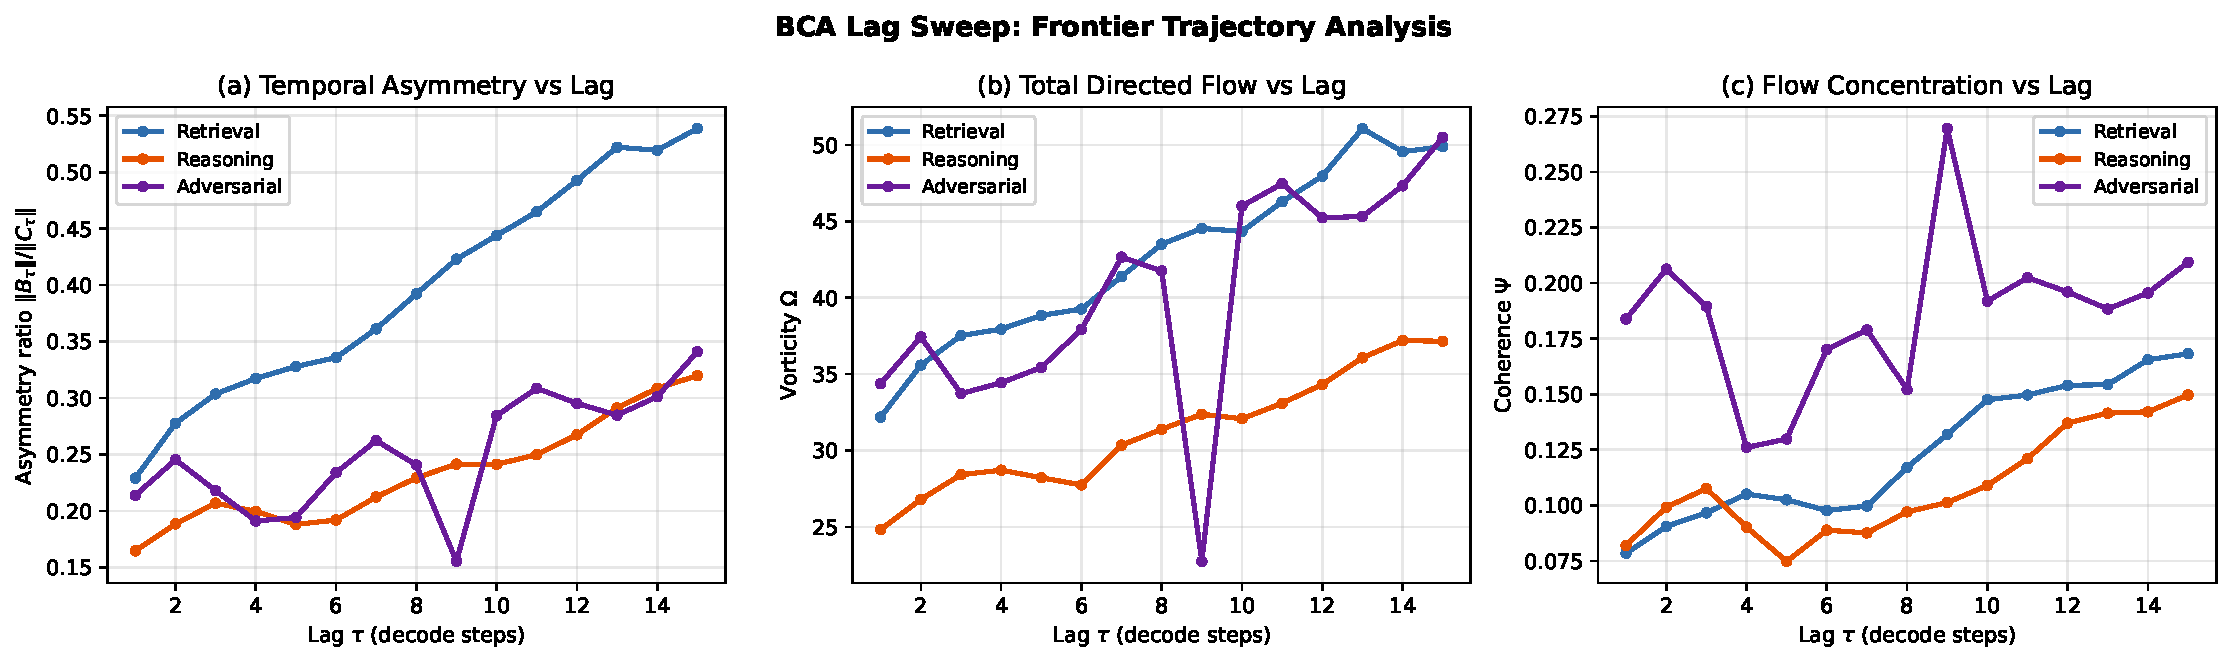
\includegraphics[width=\linewidth]{figures_ga_learning/bca_lag_sweep.pdf}
\vspace{-0.3em}
{\scriptsize\textbf{Figure:} BCA lag sweep. At lag~9 (the repetition cycle), Adversarial shows a sharp drop in directed flow and spike in coherence.}
\end{column}
\begin{column}{0.48\textwidth}
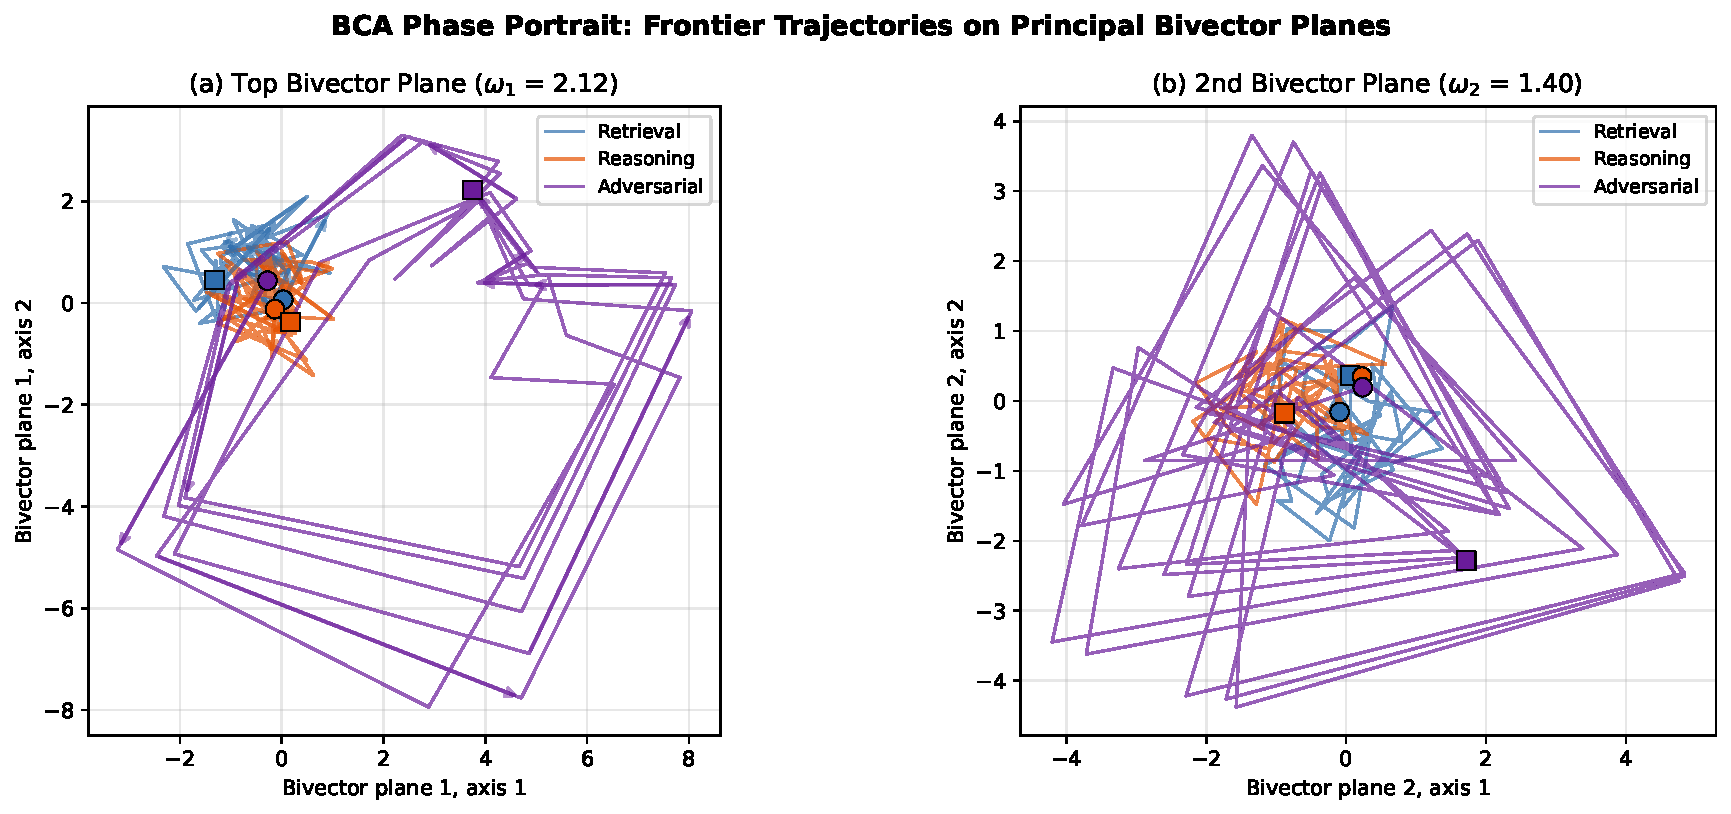
\includegraphics[width=\linewidth]{figures_ga_learning/bca_phase_portrait.pdf}
\vspace{-0.3em}
{\scriptsize\textbf{Figure:} BCA phase portrait. Trajectories projected onto the top two \emph{directed-flow} planes. Adversarial (purple) traces a large structured orbit.}
\end{column}
\end{columns}

\vspace{0.2em}
{\small Three diagnostics from $B_\tau$:}
\vspace{-0.3em}
\begin{columns}[T]
\begin{column}{0.30\textwidth}
{\scriptsize\textbf{Directed flow} $\Omega$\\Total temporal asymmetry}
\end{column}
\begin{column}{0.30\textwidth}
{\scriptsize\textbf{Coherence} $\Psi = \omega_1/\Omega$\\Flow concentration in one plane}
\end{column}
\begin{column}{0.32\textwidth}
{\scriptsize\textbf{Asymmetry ratio} $\|B\|/\|C\|$\\Directional vs.\ undirected}
\end{column}
\end{columns}

\vspace{0.2em}
{\scriptsize\textcolor{gray}{Statistical caveat: with ${\sim}60$ decode steps and $k{=}256$, the antisymmetric component $B_\tau$ can be noisy.  The diagnostics above are computed from whitened, centred trajectories and averaged across layers to mitigate finite-sample bias.}}
\end{frame}

% ── Slide: Hallucination ─────────────────────────────────────────────────────
\begin{frame}{Hallucination as geometric collapse}
\vspace{-0.3em}
\begin{columns}[c]
\begin{column}{0.44\textwidth}
\includegraphics[width=\linewidth]{figures_ga_learning/ch16_3_frontier_capacity.pdf}
\vspace{-0.3em}
{\scriptsize\textbf{Figure:} Two capacity-vs-step curves: factual (blue) vs.\ confabulated (red). Steeper slope = faster loss of sequential reasoning budget.}
\end{column}
\begin{column}{0.52\textwidth}
{\small Comparing factual vs.\ confabulated generation:}

\vspace{0.2em}
\begin{center}
\renewcommand{\arraystretch}{1.2}\footnotesize
\begin{tabular}{@{} l c c @{}}
\toprule
& \textbf{Factual} & \textbf{Confab.} \\
\midrule
Capacity decay & $-0.18$ & $-0.28$ \\
Curvature accel. & $0.186$ & $0.221$ \\
\bottomrule
\end{tabular}
\end{center}

\vspace{0.2em}
\begin{itemize}\small
  \item \textbf{56\% faster} capacity decay
  \item Curvature not just higher but \textbf{accelerating}
  \item Model loses geometric structure as it fabricates
\end{itemize}

\vspace{0.2em}
{\small\alert{In this model, hallucination has a measurable geometric signature \emph{during} generation.}}
\end{column}
\end{columns}
\end{frame}


% ╔════════════════════════════════════════════════════════════════════════════╗
% ║  PART 5: SEEING INSIDE AND STEERING                                     ║
% ╚════════════════════════════════════════════════════════════════════════════╝

\section{Seeing Inside and Steering}

% ── Slide: Online monitoring ─────────────────────────────────────────────────
\begin{frame}{Online monitoring: catching failure in real time}
\vspace{-0.3em}
\begin{columns}[c]
\begin{column}{0.46\textwidth}
\includegraphics[width=\linewidth]{figures_ga_learning/ch17_online_scores_3prompts.pdf}
\vspace{-0.3em}
{\scriptsize\textbf{Figure:} Online quality scores during generation.  The Adversarial prompt crosses the alert threshold at step~42 --- \textbf{before} human-visible repetition begins.}
\end{column}
\begin{column}{0.50\textwidth}
{\small Three scores computed at each decode step:}
\begin{enumerate}\small\setlength{\itemsep}{2pt}
  \item \textbf{Capacity growth rate} --- is the model's
    sequential budget draining too fast?
  \item \textbf{Plane diversity} --- are rotation planes
    collapsing into one?
  \item \textbf{Curvature acceleration} --- is the geometry
    becoming unstable?
\end{enumerate}

\vspace{0.3em}
{\small\alert{Empirical result (Qwen2.5-7B):} GA-based monitoring detects degradation \textbf{$\sim$8 steps before} token-level repetition becomes visible in our experiments.}
\end{column}
\end{columns}
\end{frame}

% ── Slide: Which layers matter ───────────────────────────────────────────────
\begin{frame}{Which layers matter?}
\vspace{-0.3em}
\textbf{Dependency} asks: if I perturbed this layer's output, how much would the prediction change? Measured via gradient norm: $D_l = \|\partial s / \partial H^{(l)}\|_F$.

\begin{columns}[c]
\begin{column}{0.46\textwidth}
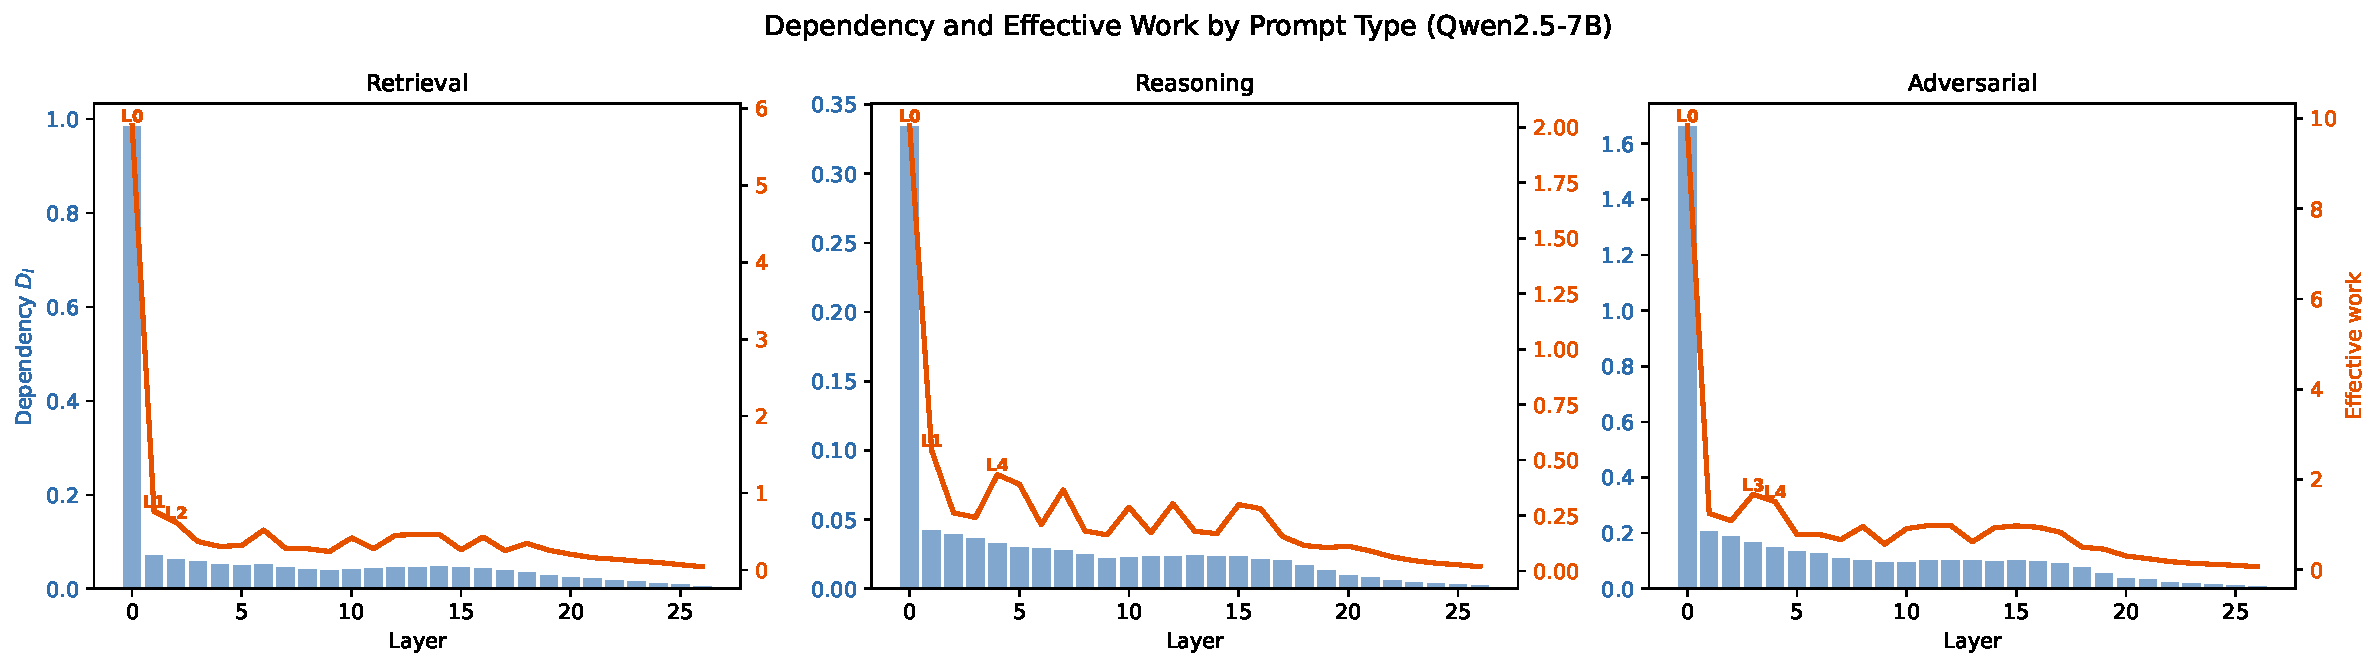
\includegraphics[width=\linewidth]{figures_ga_learning/ch12_dependency_3prompts.pdf}
\vspace{-0.3em}
{\scriptsize\textbf{Figure:} Each bar = gradient-based dependency $D_l$ per layer. Taller = the output is more sensitive to that layer's contribution.}
\end{column}
\begin{column}{0.50\textwidth}
\textbf{Effective work} combines ``how much the layer rotates'' with ``how much the output cares'':
$W_l = D_l \cdot \theta^{(l)}$

\vspace{0.2em}
\begin{itemize}\small
  \item The \textbf{loudest} layer (biggest rotation) is often \emph{not} the most important
  \item The small stretches (grade-0) sit at high-dependency layers --- geometrically quiet but \textbf{functionally decisive}
\end{itemize}

\vspace{0.2em}
{\small Effective work pinpoints where the model is both \emph{active} and \emph{consequential}.}
\end{column}
\end{columns}
\end{frame}

% ── Slide: Cayley steering ───────────────────────────────────────────────────
\begin{frame}{Cayley steering: from detection to control}
\vspace{-0.3em}
{\small The Cayley bivector between \emph{query-only} and \emph{context-augmented} hidden states tells us \textbf{where} and \textbf{in which plane} context acts:}

\vspace{-0.2em}
\begin{columns}[T]
\begin{column}{0.44\textwidth}
\includegraphics[width=\linewidth]{figures_ga_learning/ch16_steering_tau_3examples.pdf}
\vspace{-0.3em}
{\scriptsize\textbf{Figure:} $\tau^{(l)}$ per layer for three counterfactual prompts. The peak identifies where context most strongly rotates the hidden state.}
\end{column}
\begin{column}{0.54\textwidth}
\vspace{-0.3em}
\renewcommand{\arraystretch}{1.0}\scriptsize
\begin{tabular}{@{} l c c l @{}}
\toprule
\textbf{Prompt} & \textbf{Layer} & $\tau$ & \textbf{Output} \\
\midrule
Capital of Australia & 14 & 0.84 & Sydney \\
Inventor of telephone & 17 & 0.53 & Tesla \\
Boiling point & 16 & 0.77 & $250^{\circ}$C \\
\bottomrule
\end{tabular}

\vspace{0.3em}
{\small The \textbf{steering recipe}:}
\vspace{-0.2em}
\begin{enumerate}\footnotesize\setlength{\itemsep}{1pt}
  \item Compute $\tau^{(l)}$ --- find the peak layer
  \item Extract the principal plane $(v_1, v_2)$ of the Cayley bivector
  \item Apply a Rodrigues rotation by angle $\alpha$ in that plane during generation
\end{enumerate}

\vspace{0.2em}
{\small\alert{In this example, one GA object --- the Cayley bivector --- provides detection, diagnosis, and targeted intervention.}}
\end{column}
\end{columns}
\end{frame}

% ── Slide: Random steering fails ────────────────────────────────────────────
\begin{frame}{Why the plane matters: random steering fails}
\vspace{-0.3em}
\begin{columns}[c]
\begin{column}{0.48\textwidth}
\begin{center}
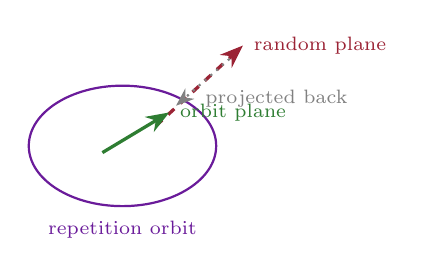
\begin{tikzpicture}[>=Stealth, scale=0.85, font=\small]
  % Orbit
  \draw[Purple, thick] (0,0) ellipse (1.4 and 0.9);
  \node[Purple, font=\scriptsize] at (0, -1.25) {repetition orbit};
  % Random arrow
  \draw[->, DRed, very thick, dashed] (0.5, 0.3) -- (1.8, 1.5)
    node[right, font=\scriptsize] {random plane};
  % Projection back
  \draw[->, gray, thick, dotted] (1.6, 1.3) -- (0.8, 0.6);
  \node[gray, font=\scriptsize] at (2.3, 0.7) {projected back};
  % Orbit plane arrow
  \draw[->, DGreen, very thick] (-0.3, -0.1) -- (0.7, 0.5)
    node[right, font=\scriptsize, DGreen] {orbit plane};
\end{tikzpicture}
\end{center}

\vspace{0.2em}
{\scriptsize In $k{=}256$ dimensions, a random 2D plane is overwhelmingly unlikely to overlap with the orbit's specific 2D subspace.}
\end{column}
\begin{column}{0.50\textwidth}
{\small \textbf{Experiment}: apply random-plane rotations at the frontier to break the adversarial repetition cycle.}

\vspace{0.2em}
\begin{itemize}\small\setlength{\itemsep}{2pt}
  \item Even at $\alpha = 0.20$ rad: \textbf{orbit persists}
  \item The model's nonlinear layers project the perturbation \textbf{back onto the attractor}
  \item \alert{Steering must target the right plane} --- the one the model actually uses
\end{itemize}

\vspace{0.2em}
{\small This negative result motivates the Cayley steering recipe: use the model's \emph{own} rotation planes.}
\end{column}
\end{columns}
\end{frame}

% ── Slide: Overcoming parametric resistance ─────────────────────────────────
\begin{frame}{When context fails: steering past parametric resistance}
\vspace{-0.3em}
\begin{columns}[T]
\begin{column}{0.46\textwidth}
\includegraphics[width=\linewidth]{figures_ga_learning/ch16_steer_resistance_sweep.pdf}
\vspace{-0.3em}
{\scriptsize\textbf{Figure:} Steering sweep on a resistant prompt. (a)~Single-layer: requires $\alpha{=}2.0$. (b)~Multi-layer: context answer at $\alpha{=}0.5$ with a narrow effective window.}
\end{column}
\begin{column}{0.52\textwidth}
{\small Context says ``Earth--Sun distance = \textbf{50 million miles}.''
Model ignores it, answers ``93 million miles.''}

\vspace{0.2em}
{\small The Cayley bivector \emph{detects} context influence ($\tau = 0.70$ at layer~16) --- the hidden states are rotated, but not enough to flip the output.}

\vspace{0.2em}
\renewcommand{\arraystretch}{1.0}\scriptsize
\begin{tabular}{@{} l c l @{}}
\toprule
\textbf{Steering} & $\alpha$ & \textbf{Result} \\
\midrule
None & --- & 93 million (parametric) \\
Single L16 & 2.0 & 1 million (context) \\
\textbf{Multi L16,17,14} & \textbf{0.5} & \textbf{50 million (exact)} \\
\bottomrule
\end{tabular}

\vspace{0.2em}
{\small\alert{Takeaway (single example):} Multi-layer Cayley steering at moderate $\alpha$ can override parametric resistance that context alone cannot --- a geometrically targeted nudge in the model's own rotation planes.}
\end{column}
\end{columns}
\end{frame}


% ╔════════════════════════════════════════════════════════════════════════════╗
% ║  THE BIG PICTURE                                                        ║
% ╚════════════════════════════════════════════════════════════════════════════╝

\section{The Big Picture}

% ── Slide: Three fields ──────────────────────────────────────────────────────
\begin{frame}{A transformer is a geometric field system}

The entire framework is captured in \textbf{three fields} over a discrete grid:

\vspace{0.5em}
\[
\begin{aligned}
  H &: \mathcal{G} \;\longrightarrow\; \mathbb{R}^k
    &&\text{(hidden-state field)} \\[6pt]
  R &: \mathcal{G} \;\longrightarrow\; \mathrm{Spin}(k)
    &&\text{(rotor field)} \\[6pt]
  \Omega &: \mathcal{G} \;\longrightarrow\; \mathfrak{so}(k)
    &&\text{(curvature field)}
\end{aligned}
\]

\vspace{0.8em}
\begin{center}
\large\color{Navy}
\emph{Vectors \;\;$\longrightarrow$\;\; Rotations \;\;$\longrightarrow$\;\; Curvature}
\end{center}
\end{frame}

% ── Slide: What was invisible ────────────────────────────────────────────────
\begin{frame}{What GA reveals that norms cannot}
\vspace{-0.3em}
Scalar summaries tell you \textbf{how much}.
GA tells you \textbf{how much} and \textbf{in which direction}.

\vspace{0.3em}
\begin{columns}[T]
\begin{column}{0.48\textwidth}
\textbf{Static} (single forward pass):
\begin{enumerate}\small
  \item Which planes each layer rotates in
  \item Which planes the curvature acts in
  \item Which planes layers fail to commute in
  \item Which planes the output depends on
\end{enumerate}
\end{column}
\begin{column}{0.48\textwidth}
\textbf{Dynamic} (during generation):
\begin{enumerate}\small\setcounter{enumi}{4}
  \item How rotation planes drift or collapse
  \item \textbf{Directed flow} via BCA (temporal order)
  \item Whether capacity decay signals hallucination
  \item Real-time monitoring \emph{before} failure
\end{enumerate}
\end{column}
\end{columns}

\vspace{0.3em}
\begin{center}
\fcolorbox{Navy}{LBlue}{\parbox{0.7\textwidth}{\centering\small
\textbf{A transformer is a discrete geometric field system\\
whose computation is governed by rotations and curvature.}}}
\end{center}
\end{frame}

% ── Slide: Summary ───────────────────────────────────────────────────────────
\begin{frame}{Summary}
\vspace{-0.6em}
\renewcommand{\arraystretch}{1.0}
\begin{center}\scriptsize
\begin{tabular}{@{} l l l @{}}
\toprule
\textbf{Concept} & \textbf{Intuition} & \textbf{GA object} \\
\midrule
Versor decomp. & Layer rotates vs.\ stretches & $T = R \cdot P$ \\
Bivector field & Which directions reshuffled & $B^{(l)} \in \mathfrak{so}(k)$ \\
Commutator & Does layer order matter? & $[B^{(l)}, B^{(l+1)}]$ \\
Capacity & Sequential computation budget & $C_{\text{acc}} = \sum \|[\cdot]\|_F$ \\
Holonomy & Layer--context entanglement & $R_{\text{loop}}$ \\
Dependency & Which layers matter & $D_l = \|\partial s / \partial H^{(l)}\|_F$ \\
BCA & Directed temporal flow & $B_\tau = (M - M^\top)/2$ \\
Monitoring & Real-time failure detection & Quality scores at frontier \\
\bottomrule
\end{tabular}
\end{center}

\vspace{0.1em}
\textbf{Key takeaways:}\vspace{-0.3em}
\begin{enumerate}\small\setlength{\itemsep}{1pt}
  \item Layers are predominantly \textbf{rotations}; non-commutativity underlies sequential reasoning
  \item \textbf{Curvature} reveals layer--context entanglement
  \item \textbf{BCA} recovers temporal direction that PCA discards
  \item Hallucination has a measurable \textbf{geometric signature} (in our experiments)
  \item The Cayley bivector enables \textbf{plane-specific intervention}
\end{enumerate}
\end{frame}

% ── Slide: Thank you / Q&A ──────────────────────────────────────────────────
{
\setbeamercolor{background canvas}{bg=Navy}
\setbeamercolor{normal text}{fg=white}
\begin{frame}[plain, c]
\usebeamercolor[fg]{normal text}
\begin{center}
{\Huge Questions?}

\vspace{0.8em}
{\large How LLMs Process Information: A Geometric View}

\vspace{0.4em}
{\small Agus Sudjianto}

\vspace{0.4em}
{\scriptsize Based on \emph{Learning Geometric Algebra Through Transformer Geometry}}

\vspace{0.2em}
{\scriptsize\url{https://github.com/asudjianto-xml/layer-time-geometry}}

\vspace{0.4em}
{\scriptsize
Model: Qwen2.5-7B (28 layers, whitened to $k = 256$) ~$\cdot$~
Library: \texttt{layer\_time\_ga}}
\end{center}
\end{frame}
}

\end{document}
